
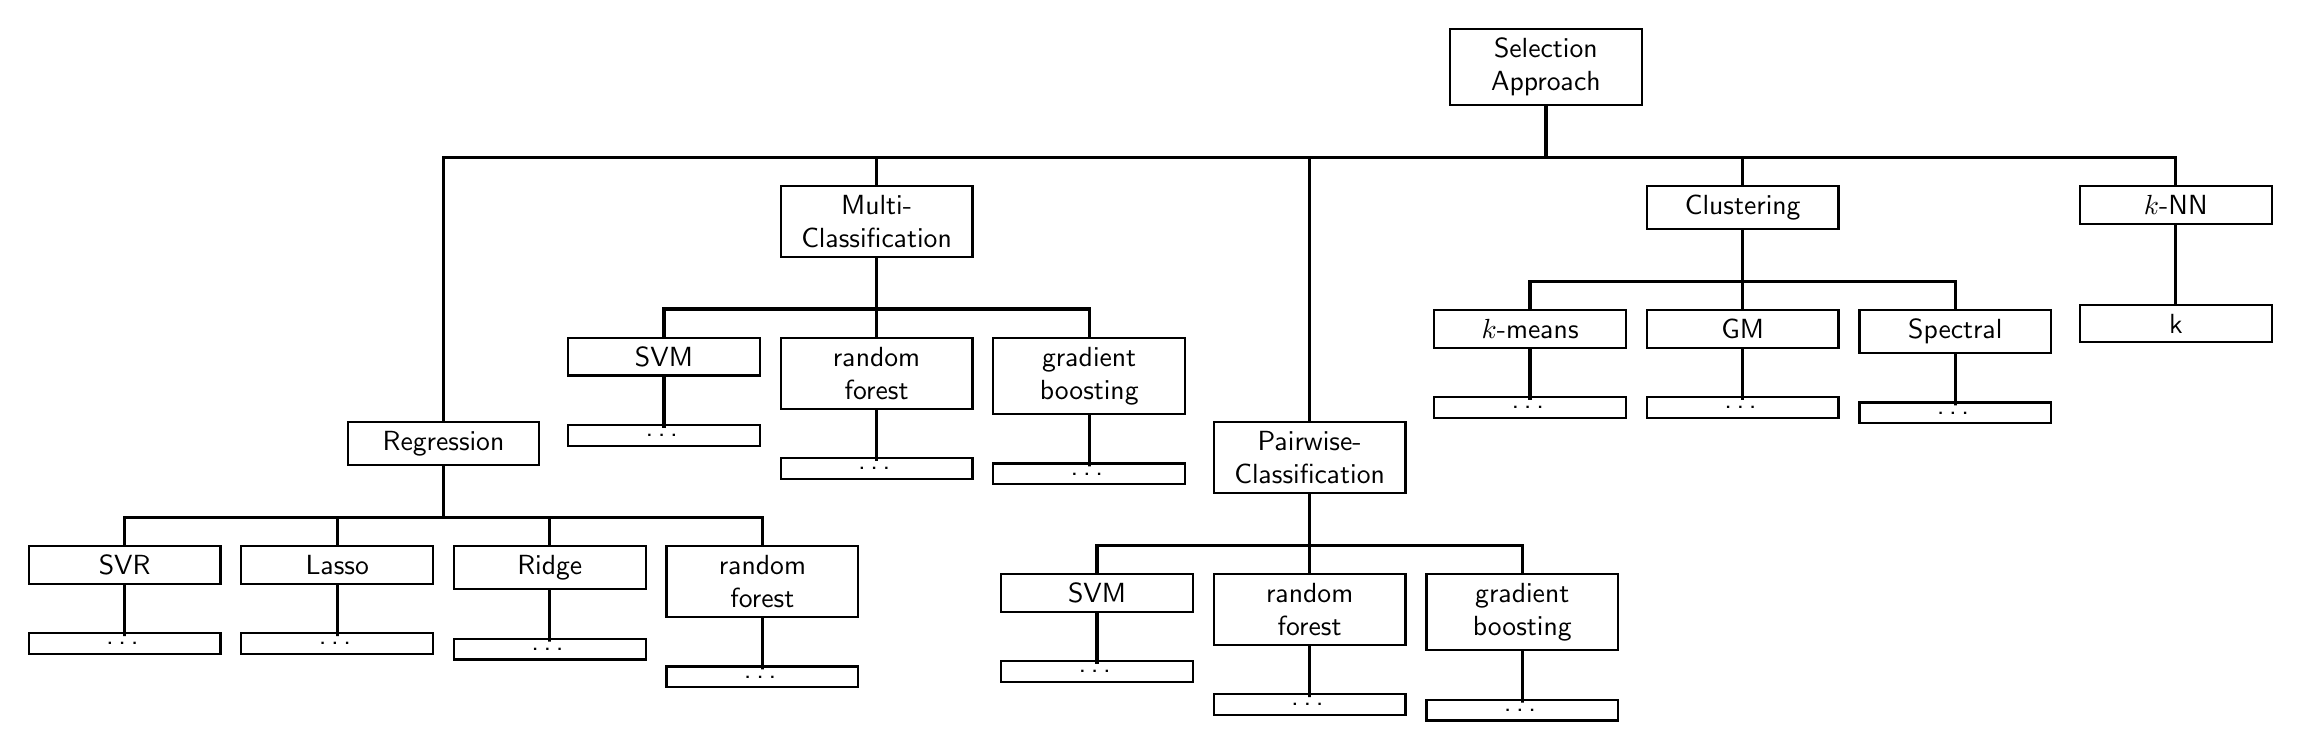
\begin{tikzpicture}[
% Label style
    label distance=3mm,
    every label/.style={blue},
% Event style
    event/.style={rectangle,thick,draw,text width=2.2cm,
		text centered,font=\sffamily,anchor=north},
% Children and edges style
    edge from parent/.style={very thick,draw=black},
    edge from parent path={(\tikzparentnode.south) -- ++(0,-.65cm) -| (\tikzchildnode.north)},
	level 1/.style={sibling distance=7cm, level distance=1.0cm, growth parent anchor=south,nodes=event},
    level 2/.style={sibling distance=6.0cm, level distance=1.0cm},
    level 3/.style={sibling distance=2.4cm,level distance=0.6cm},
    %level 4/.style={sibling distance=5cm},
    %level 5/.style={sibling distance=5cm}
    %level 6/.style={sibling distance=6cm}
%%  For compatability with PGF CVS add the absolute option:
%   absolute
    ]
%% Draw events and edges
    \node (comp) [event] {Selection Approach} 
       child{
       	  node [sibling distance=8.9cm, yshift=-3.0cm] {Regression}
       	  child [sibling distance=2.7cm] {
				node {SVR}
				child { node {\ldots}}	
		  }				       	  
  		  child [sibling distance=2.7cm] {
  				node {Lasso}   
  				child { node {\ldots}}	
	       }
	      child [sibling distance=2.7cm] {
  				node {Ridge}   
  				child { node {\ldots}}	
	       } 
	       child [sibling distance=2.7cm] {
  				node {random\\ forest}  
  				child { node {\ldots}}	 
	       } 
       }
        child{
       	  node [sibling distance=8.9cm, xshift=-1.5cm]  {Multi-Classification}
       	  child [sibling distance=2.7cm] {
				node  {SVM}
				child { node {\ldots}}	
		  }				       	  
  		  child [sibling distance=2.7cm] {
  				node {random\\ forest}   
  				child { node {\ldots}}	
	       }
	      child [sibling distance=2.7cm] {
  				node {gradient boosting}   
  				child { node {\ldots}}	
	       }
	     } 
	     child{
       	  node [sibling distance=8.9cm, yshift=-3.0cm, xshift=-3.0cm] {Pairwise-Classification}
       	  child [sibling distance=2.7cm] {
				node  {SVM}
				child { node {\ldots}}	
		  }				       	  
  		  child [sibling distance=2.7cm] {
  				node {random\\ forest}   
  				child { node {\ldots}}	
	       }
	      child [sibling distance=2.7cm] {
  				node {gradient boosting}   
  				child { node {\ldots}}	
	       }
	      }
	      child{
       	  node [sibling distance=8.9cm, xshift=-4.5cm] {Clustering}
       	  child [sibling distance=2.7cm] {
				node {$k$-means}
				child { node {\ldots}}	
		  }				       	  
  		  child [sibling distance=2.7cm] {
  				node {GM}   
  				child { node {\ldots}}	
	       }
	      child [sibling distance=2.7cm] {
  				node {Spectral}   
  				child { node {\ldots}}	
	       }
	      } 
	      child{
       	  node [sibling distance=8.9cm, xshift=-6.0cm] {$k$-NN}
       	  child [sibling distance=2.7cm] {
				node  {k}
		  	}
       };
	     
\end{tikzpicture}
